\apendice{Especificación de Requisitos}

\section{Introducción}
Esta sección contendrá los requisitos y objetivos del proyecto. Consistirá en breves descripciones de los objetivos principales, que a su vez se dividen en objetivos más pequeños.

\section{Objetivos generales}
Los objetivos que se persiguen en este proyecto son:
\begin{itemize}
	\item Construcción de los clasificadores base \textbf{DisturbingNeighbors}, \textbf{RandomOracles}, \textbf{RotationForest}: Se construirán tres clasificadores, cuyo objetivo sera conseguir clasificar un conjunto de datos de manera más eficaz que otros clasificadores ya existentes en Sklearn.
	\item Construcción de ensembles: Se construyen ensembles de los clasificadores base para mejorar su efectividad. 
\end{itemize}

\section{Catalogo de requisitos}
El proyecto consiste en:
\begin{itemize}
	\item Entrenar los clasificadores base.
	\begin{itemize}
		\item Entrenar  \textbf{DisturbingNeighbors}.
		\item Entrenar  \textbf{RandomOracles}.
		\item Entrenar  \textbf{RotationForest}.
	\end{itemize}
	\item Predecir los clasificadores base.
	\begin{itemize}
		\item Predecir  \textbf{DisturbingNeighbors}.
		\item Predecir  \textbf{RandomOracles}.
		\item Predecir  \textbf{RotationForest}.
	\end{itemize}
	\item Predecir probabilidades de los clasificadores base.
	\begin{itemize}
		\item Predecir probabilidades de \textbf{DisturbingNeighbors}.
		\item Predecir probabilidades de  \textbf{RandomOracles}.
		\item Predecir probabilidades de  \textbf{RotationForest}.
	\end{itemize}
	\item Entrenar los ensembles.
	\item Predecir los ensembles.
	\item Predecir probabilidades de los ensembles.
\end{itemize}
\section{Especificación de requisitos}
\begin{itemize}
	\item RF-1: Entrenar los clasificadores base.
	\begin{itemize}
		\item RF-1.1: Entrenar  \textbf{DisturbingNeighbors}.
		\item RF-1.2: Entrenar  \textbf{RandomOracles}.
		\item RF-1.3: Entrenar  \textbf{RotationForest}.
	\end{itemize}
	\item RF-2: Predecir los clasificadores base.
	\begin{itemize}
		\item RF-2.1: Predecir  \textbf{DisturbingNeighbors}.
		\item RF-2.2: Predecir  \textbf{RandomOracles}.
		\item RF-2.3: Predecir  \textbf{RotationForest}.
	\end{itemize}
	\item RF-3: Predecir probabilidades de los clasificadores base.
	\begin{itemize}
		\item RF-3.1: Predecir probabilidades de \textbf{DisturbingNeighbors}.
		\item RF-3.2: Predecir probabilidades de  \textbf{RandomOracles}.
		\item RF-3.3: Predecir probabilidades de  \textbf{RotationForest}.
	\end{itemize}
	\item RF-4: Entrenar los ensembles.
	\item RF-5: Predecir los ensembles.
	\item RF-6: Predecir probabilidades de los ensembles.
\end{itemize} 

\subsection{Diagrama de casos de uso}
El diagrama que contiene los caso de uso de nuestro proyecto esta contenido en la figura \ref{fig:DiagramCaseUseGeneral}.	

\begin{figure}
\centering
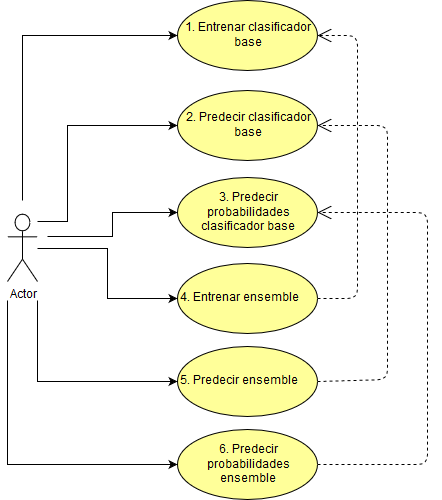
\includegraphics[width=.65\textwidth]{DiagramCaseUseGeneral}
\caption{Diagrama general de casos de uso.}
\label{fig:DiagramCaseUseGeneral}
\end{figure}

Este caso de uso se extiende en otros tres, que serían el de entrenamiento de los clasificadores base \ref{fig:DiagramCase1}, otro de predicción de los clasificadores base \ref{fig:DiagramCase2}, y el último de predecir probabilidades de los clasificadores base \ref{fig:DiagramCase3}.	

\begin{figure}
\centering
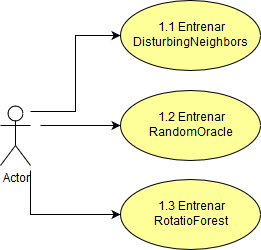
\includegraphics[width=0.5\textwidth]{DiagramCase1}
\caption{Diagrama de entrenamiento de los clasificadores.}
\label{fig:DiagramCase1}
\end{figure}

\begin{figure}
\centering
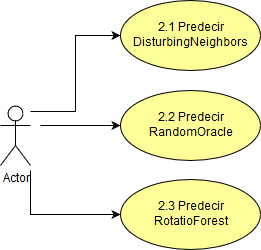
\includegraphics[width=0.5\textwidth]{DiagramCase2}
\caption{Diagrama de predicción de los clasificadores.}
\label{fig:DiagramCase2}
\end{figure}

\begin{figure}
\centering
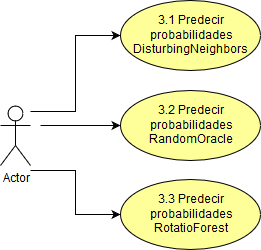
\includegraphics[width=0.5\textwidth]{DiagramCase3}
\caption{Diagrama de probabilidades de los clasificadores.}
\label{fig:DiagramCase3}
\end{figure}

A partir del diagrama principal y los demás diagramas, se han diseñado las siguientes tablas de los diagramas de casos de uso, se muestran en las siguientes figuras, \ref{tab:tablacaso1}, \ref{tab:tablacaso2}, \ref{tab:tablacaso3}, \ref{tab:tablacaso4}, \ref{tab:tablacaso5}, \ref{tab:tablacaso6} y este se subdivide en \ref{tab:tablacaso1.1}, \ref{tab:tablacaso1.2}, \ref{tab:tablacaso1.3}, \ref{tab:tablacaso2.1}, \ref{tab:tablacaso2.2} y \ref{tab:tablacaso2.3}.

\begin{table}[]
\centering
\caption{Tabla del caso de uso 1}
\label{tab:tablacaso1}
\begin{tabular}{@{}
>{\columncolor[HTML]{FFFFFF}}p {.25\textwidth} p {.75\textwidth}@{}}
\toprule
\textbf{Caso de uso 1}   & Entrenar los clasificadores base \\ \midrule
\textbf{Versión}         & 1.0                                                                                                                                                                           \\ \midrule
\textbf{Autor}           & Eduardo Tubilleja Calvo                                                                                                                                                             \\ \midrule
\textbf{Requisitos}      & \begin{tabular}[c]{@{}l@{}}RF-1\\ RF-1.1\\ RF-1.2\\ RF-1.3\end{tabular}                                                                                                                  \\ \midrule
\textbf{Descripción}     & \begin{tabular}[c]{@{}l@{}}El usuario podrá entrenar un conjunto de datos a través\\ de un clasificador base.
\end{tabular}            \\ \midrule
\textbf{Precondiciones}  & No tiene                                                                                                                                                                        \\ \midrule
\textbf{Acciones}        & \begin{tabular}[c]{@{}l@{}}1 Ejecutar Jupyter.\\ 2 Seleccionar el notebook.\\ 3 Crear el conjunto de datos.\\ 4 Seleccionar el clasificador.\\ 5 Entrenar el conjunto de datos.
\end{tabular} \\ \midrule
\textbf{Postcondiciones} & El clasificador base entrenado.                                                                                                                                   \\ \midrule
\textbf{Excepciones}     & Ninguna
\\ \midrule
\textbf{Importancia}     & Baja                                                                                                                                                                            \\ \bottomrule
\end{tabular}
\end{table}

\begin{table}[]
\centering
\caption{Tabla del caso de uso 2}
\label{tab:tablacaso2}
\begin{tabular}{@{}
>{\columncolor[HTML]{FFFFFF}}p {.25\textwidth} p {.75\textwidth}@{}}
\toprule
\textbf{Caso de uso 1}   & Predecir los clasificadores base \\ \midrule
\textbf{Versión}         & 1.0                                                                                                                                                                           \\ \midrule
\textbf{Autor}           & Eduardo Tubilleja Calvo                                                                                                                                                             \\ \midrule
\textbf{Requisitos}      & \begin{tabular}[c]{@{}l@{}}RF-2\\ RF-2.1\\ RF-2.2\\ RF-2.3\end{tabular}                                                                                                                  \\ \midrule
\textbf{Descripción}     & \begin{tabular}[c]{@{}l@{}}El usuario podrá predecir un conjunto de datos a través\\ de un clasificador base.
\end{tabular}            \\ \midrule
\textbf{Precondiciones}  & Haber entrenado el clasificador.                                                                                                                                                                        \\ \midrule
\textbf{Acciones}        & \begin{tabular}[c]{@{}l@{}}1 Ejecutar Jupyter.\\ 2 Seleccionar el notebook.\\ 3 Crear el conjunto de datos.\\ 4 Seleccionar el clasificador.\\ 5 Predecir el conjunto de datos.
\end{tabular} \\ \midrule
\textbf{Postcondiciones} & El clasificador base tiene una predicción.                                                                                                                                   \\ \midrule
\textbf{Excepciones}     & Ninguna
\\ \midrule
\textbf{Importancia}     & Baja                                                                                                                                                                            \\ \bottomrule
\end{tabular}
\end{table}

\begin{table}[]
\centering
\caption{Tabla del caso de uso 3}
\label{tab:tablacaso3}
\begin{tabular}{@{}
>{\columncolor[HTML]{FFFFFF}}p {.25\textwidth} p {.75\textwidth}@{}}
\toprule
\textbf{Caso de uso 1}   & Predecir la probabilidad de los clasificadores base \\ \midrule
\textbf{Versión}         & 1.0                                                                                                                                                                           \\ \midrule
\textbf{Autor}           & Eduardo Tubilleja Calvo                                                                                                                                                             \\ \midrule
\textbf{Requisitos}      & \begin{tabular}[c]{@{}l@{}}RF-3\\ RF-3.1\\ RF-3.2\\ RF-3.3\end{tabular}                                                                                                                  \\ \midrule
\textbf{Descripción}     & \begin{tabular}[c]{@{}l@{}}El usuario podrá predecir las probabilidades de un\\ conjunto de datos a través de un clasificador base.
\end{tabular}            \\ \midrule
\textbf{Precondiciones}  & Haber entrenado el clasificador.                                                                                                                                                                        \\ \midrule
\textbf{Acciones}        & \begin{tabular}[c]{@{}l@{}}1 Ejecutar Jupyter.\\ 2 Seleccionar el notebook.\\ 3 Crear el conjunto de datos.\\ 4 Seleccionar el clasificador.\\ 5 Predecir probabilidades del conjunto de datos.
\end{tabular} \\ \midrule
\textbf{Postcondiciones} & El clasificador base saca unas probabilidades.                                                                                                                                   \\ \midrule
\textbf{Excepciones}     & Ninguna
\\ \midrule
\textbf{Importancia}     & Baja                                                                                                                                                                            \\ \bottomrule
\end{tabular}
\end{table}

\begin{table}[]
\centering
\caption{Tabla del caso de uso 4}
\label{tab:tablacaso4}
\begin{tabular}{@{}
>{\columncolor[HTML]{FFFFFF}}p {.25\textwidth} p {.75\textwidth}@{}}
\toprule
\textbf{Caso de uso 1}   & Entrenar ensemble \\ \midrule
\textbf{Versión}         & 1.0                                                                                                                                                                           \\ \midrule
\textbf{Autor}           & Eduardo Tubilleja Calvo                                                                                                                                                             \\ \midrule
\textbf{Requisitos}      & \begin{tabular}[c]{@{}l@{}}RF-4\end{tabular}                                                                                                                  \\ \midrule
\textbf{Descripción}     & \begin{tabular}[c]{@{}l@{}}El usuario podrá entrenar un conjunto de datos, a\\ través de un ensemble de clasificadores base.
\end{tabular}            \\ \midrule
\textbf{Precondiciones}  & No tiene                                                                                                                                                                        \\ \midrule
\textbf{Acciones}        & \begin{tabular}[c]{@{}l@{}}1 Ejecutar Jupyter.\\ 2 Seleccionar el notebook.\\ 3 Crear el conjunto de datos.\\ 4 Seleccionar el ensemble.\\ 5 Entrenar el conjunto de datos.
\end{tabular} \\ \midrule
\textbf{Postcondiciones} & El ensemble de clasificadores base entrenado.                                                                                                                                   \\ \midrule
\textbf{Excepciones}     & Ninguna
\\ \midrule
\textbf{Importancia}     & Baja                                                                                                                                                                            \\ \bottomrule
\end{tabular}
\end{table}

\begin{table}[]
\centering
\caption{Tabla del caso de uso 5}
\label{tab:tablacaso5}
\begin{tabular}{@{}
>{\columncolor[HTML]{FFFFFF}}p {.25\textwidth} p {.75\textwidth}@{}}
\toprule
\textbf{Caso de uso 1}   & Predecir ensemble \\ \midrule
\textbf{Versión}         & 1.0                                                                                                                                                                           \\ \midrule
\textbf{Autor}           & Eduardo Tubilleja Calvo                                                                                                                                                             \\ \midrule
\textbf{Requisitos}      & \begin{tabular}[c]{@{}l@{}}RF-5\end{tabular}                                                                                                                  \\ \midrule
\textbf{Descripción}     & \begin{tabular}[c]{@{}l@{}}El usuario podrá predecir un conjunto de datos, a través\\ de un ensemble de clasificadores base.
\end{tabular}            \\ \midrule
\textbf{Precondiciones}  & Haber entrenado el ensemble.
\\ \midrule
\textbf{Acciones}        & \begin{tabular}[c]{@{}l@{}}1 Ejecutar Jupyter.\\ 2 Seleccionar el notebook.\\ 3 Crear el conjunto de datos.\\ 4 Seleccionar el ensemble.\\ 5 Predecir el conjunto de datos.
\end{tabular} \\ \midrule
\textbf{Postcondiciones} & El ensemble de clasificadores base con predicciones.                                                                                                                                   \\ \midrule
\textbf{Excepciones}     & Ninguna
\\ \midrule
\textbf{Importancia}     & Baja                                                                                                                                                                            \\ \bottomrule
\end{tabular}
\end{table}

\begin{table}[]
\centering
\caption{Tabla del caso de uso 6}
\label{tab:tablacaso6}
\begin{tabular}{@{}
>{\columncolor[HTML]{FFFFFF}}p {.25\textwidth} p {.75\textwidth}@{}}
\toprule
\textbf{Caso de uso 1}   & Predecir ensemble \\ \midrule
\textbf{Versión}         & 1.0                                                                                                                                                                           \\ \midrule
\textbf{Autor}           & Eduardo Tubilleja Calvo                                                                                                                                                             \\ \midrule
\textbf{Requisitos}      & \begin{tabular}[c]{@{}l@{}}RF-6\end{tabular}                                                                                                                  \\ \midrule
\textbf{Descripción}     & \begin{tabular}[c]{@{}l@{}}El usuario podrá predecir las probabilidades de un\\ conjunto de datos, a través de un ensemble de\\ clasificadores base.
\end{tabular}            \\ \midrule
\textbf{Precondiciones}  & Haber entrenado el ensemble.                                                                                                                                                                        \\ \midrule
\textbf{Acciones}        & \begin{tabular}[c]{@{}l@{}}1 Ejecutar Jupyter.\\ 2 Seleccionar el notebook.\\ 3 Crear el conjunto de datos.\\ 4 Seleccionar el ensemble.\\ 5 Predecir probabilidades del conjunto de datos.
\end{tabular} \\ \midrule
\textbf{Postcondiciones} & El ensemble de clasificadores base con probabilidades.                                                                                                                                   \\ \midrule
\textbf{Excepciones}     & Ninguna
\\ \midrule
\textbf{Importancia}     & Baja                                                                                                                                                                            \\ \bottomrule
\end{tabular}
\end{table}

\begin{table}[]
\centering
\caption{Tabla del caso de uso 1.1}
\label{tab:tablacaso1.1}
\begin{tabular}{@{}
>{\columncolor[HTML]{FFFFFF}}p {.25\textwidth} p {.75\textwidth}@{}}
\toprule
\textbf{Caso de uso 1}   & Entrenar Disturbing Neighbors \\ \midrule
\textbf{Versión}         & 1.0                                                                                                                                                                           \\ \midrule
\textbf{Autor}           & Eduardo Tubilleja Calvo                                                                                                                                                             \\ \midrule
\textbf{Requisitos}      & \begin{tabular}[c]{@{}l@{}}RF-1.1\end{tabular}                                                                                                                  \\ \midrule
\textbf{Descripción}     & \begin{tabular}[c]{@{}l@{}}El usuario podrá entrenar un conjunto de datos a través\\ del clasificador base Disturbing Neighbors.
\end{tabular}            \\ \midrule
\textbf{Precondiciones}  & No tiene                                                                                                                                                                        \\ \midrule
\textbf{Acciones}        & \begin{tabular}[c]{@{}l@{}}1 Calcular número de características.\\ 2 Seleccionar aleatoriamente las características.\\ 3 Seleccionar aleatoriamente las instancias.\\ 4 Calcular la matriz de los vecinos molestones.\\ 5 Calcular los vecinos mas cercanos.\\ 7 Concatenar el conjunto de datos con la matriz de\\ vecinos más cercanos.\\ 8 Entrenar.
\end{tabular} \\ \midrule
\textbf{Postcondiciones} & Disturbing Neigbors entrenado.                                                                                                                                   \\ \midrule
\textbf{Excepciones}     & Número de instancias menor que el número de  vecinos molestones
\\ \midrule
\textbf{Importancia}     & Alta                                                                                                                                                                            \\ \bottomrule
\end{tabular}
\end{table}

\begin{table}[]
\centering
\caption{Tabla del caso de uso 1.2}
\label{tab:tablacaso1.2}
\begin{tabular}{@{}
>{\columncolor[HTML]{FFFFFF}}p {.25\textwidth} p {.75\textwidth}@{}}
\toprule
\textbf{Caso de uso 1}   & Entrenar Random Oracle \\ \midrule
\textbf{Versión}         & 1.0                                                                                                                                                                           \\ \midrule
\textbf{Autor}           & Eduardo Tubilleja Calvo                                                                                                                                                             \\ \midrule
\textbf{Requisitos}      & \begin{tabular}[c]{@{}l@{}}RF-1.2\end{tabular}                                                                                                                  \\ \midrule
\textbf{Descripción}     & \begin{tabular}[c]{@{}l@{}}El usuario podrá entrenar un conjunto de datos a través\\ del clasificador base Random Oracle.
\end{tabular}            \\ \midrule
\textbf{Precondiciones}  & No tiene                                                                                                                                                                        \\ \midrule
\textbf{Acciones}        & \begin{tabular}[c]{@{}l@{}}1 Comprobar si es Single-Label o Multi-Label.\\ 2 Seleccionar aleatoriamente las instancias.\\ 3 Calcular la matriz de los oráculos.\\ 4 Calcular los oráculos mas cercanos.\\ 5 Entrenar cada oráculo.
\end{tabular} \\ \midrule
\textbf{Postcondiciones} & Random Oracle entrenado.                                                                                                                                   \\ \midrule
\textbf{Excepciones}     & Ninguna
\\ \midrule
\textbf{Importancia}     & Baja
 \\ \bottomrule
\end{tabular}
\end{table}

\begin{table}[]
\centering
\caption{Tabla del caso de uso 1.3}
\label{tab:tablacaso1.3}
\begin{tabular}{@{}
>{\columncolor[HTML]{FFFFFF}}p {.25\textwidth} p {.75\textwidth}@{}}
\toprule
\textbf{Caso de uso 1}   & Entrenar Rotation Forest \\ \midrule
\textbf{Versión}         & 1.0                                                                                                                                                                           \\ \midrule
\textbf{Autor}           & Eduardo Tubilleja Calvo                                                                                                                                                             \\ \midrule
\textbf{Requisitos}      & \begin{tabular}[c]{@{}l@{}}RF-1.3\end{tabular}                                                                                                                  \\ \midrule
\textbf{Descripción}     & \begin{tabular}[c]{@{}l@{}}El usuario podrá entrenar un conjunto de datos a través\\ del clasificador base Rotation Forest.
\end{tabular}            \\ \midrule
\textbf{Precondiciones}  & No tiene                                                                                                                                                                        \\ \midrule
\textbf{Acciones}        & \begin{tabular}[c]{@{}l@{}}1 Seleccionar aleatoriamente las características.\\ 2 Seleccionar las distintas clases.\\ 3 Elegir una muestra de las clases seleccionada.\\ 4 Obtener las instancias de la muestra de clases.\\ 5 Dividir el conjunto de datos en partes.\\ 6 Entrenar PCA para cada una de los subgrupos.\\ 7 Transformar cada subgrupo con su respectivo PCA.\\ 8 Concatenar todos los subgrupos.\\ 9 Entrenar.
\end{tabular} \\ \midrule
\textbf{Postcondiciones} & Rotation Forest entrenado.                                                                                                                                   \\ \midrule
\textbf{Excepciones}     & Ninguna
\\ \midrule
\textbf{Importancia}     & Baja
 \\ \bottomrule
\end{tabular}
\end{table}

\begin{table}[]
\centering
\caption{Tabla del caso de uso 2.1}
\label{tab:tablacaso2.1}
\begin{tabular}{@{}
>{\columncolor[HTML]{FFFFFF}}p {.25\textwidth} p {.75\textwidth}@{}}
\toprule
\textbf{Caso de uso 1}   & Predecir Disturbing Neighbors \\ \midrule
\textbf{Versión}         & 1.0                                                                                                                                                                           \\ \midrule
\textbf{Autor}           & Eduardo Tubilleja Calvo                                                                                                                                                             \\ \midrule
\textbf{Requisitos}      & \begin{tabular}[c]{@{}l@{}}RF-2.1\end{tabular}                                                                                                                  \\ \midrule
\textbf{Descripción}     & \begin{tabular}[c]{@{}l@{}}El usuario podrá predecir un conjunto de datos a través\\ del clasificador base Disturbing Neighbors.
\end{tabular}            \\ \midrule
\textbf{Precondiciones}  & Haber entrenado el clasificador.                                                                                                                                                                        \\ \midrule
\textbf{Acciones}        & \begin{tabular}[c]{@{}l@{}}1 Calcular los vecinos mas cercanos.\\ 2 Concatenar el conjunto de datos con la matriz de\\ vecinos más cercanos.\\ 3 Predecir.
\end{tabular} \\ \midrule
\textbf{Postcondiciones} & Disturbing Neigbors tiene una predicción.                                                                                                                                   \\ \midrule
\textbf{Excepciones}     & Ninguna
\\ \midrule
\textbf{Importancia}     & Baja                                                                                                                                                                            \\ \bottomrule
\end{tabular}
\end{table}

\begin{table}[]
\centering
\caption{Tabla del caso de uso 2.2}
\label{tab:tablacaso2.2}
\begin{tabular}{@{}
>{\columncolor[HTML]{FFFFFF}}p {.25\textwidth} p {.75\textwidth}@{}}
\toprule
\textbf{Caso de uso 1}   & Predecir Random Oracle \\ \midrule
\textbf{Versión}         & 1.0                                                                                                                                                                           \\ \midrule
\textbf{Autor}           & Eduardo Tubilleja Calvo                                                                                                                                                             \\ \midrule
\textbf{Requisitos}      & \begin{tabular}[c]{@{}l@{}}RF-2.2\end{tabular}                                                                                                                  \\ \midrule
\textbf{Descripción}     & \begin{tabular}[c]{@{}l@{}}El usuario podrá predecir un conjunto de datos a través\\ del clasificador base Random Oracle.
\end{tabular}            \\ \midrule
\textbf{Precondiciones}  & Haber entrenado el clasificador.                                                                                                                                                                        \\ \midrule
\textbf{Acciones}        & \begin{tabular}[c]{@{}l@{}}1 Concatenar el conjunto de datos con los oráculos más\\ cercanos.\\ 2 Predecir instancias con el oráculo correspondiente más\\ cercano.
\end{tabular} \\ \midrule
\textbf{Postcondiciones} & Random Oracle tiene una predicción.                                                                                                                                   \\ \midrule
\textbf{Excepciones}     & Ninguna
\\ \midrule
\textbf{Importancia}     & Baja                                                                                                                                                                            \\ \bottomrule
\end{tabular}
\end{table}

\begin{table}[]
\centering
\caption{Tabla del caso de uso 2.3}
\label{tab:tablacaso2.3}
\begin{tabular}{@{}
>{\columncolor[HTML]{FFFFFF}}p {.25\textwidth} p {.75\textwidth}@{}}
\toprule
\textbf{Caso de uso 1}   & Predecir Rotation Forest \\ \midrule
\textbf{Versión}         & 1.0                                                                                                                                                                           \\ \midrule
\textbf{Autor}           & Eduardo Tubilleja Calvo                                                                                                                                                             \\ \midrule
\textbf{Requisitos}      & \begin{tabular}[c]{@{}l@{}}RF-2.3\end{tabular}                                                                                                                  \\ \midrule
\textbf{Descripción}     & \begin{tabular}[c]{@{}l@{}}El usuario podrá predecir un conjunto de datos a través\\ del clasificador base Rotation Forest.
\end{tabular}            \\ \midrule
\textbf{Precondiciones}  & Haber entrenado el clasificador.                                                                                                                                                                        \\ \midrule
\textbf{Acciones}        & \begin{tabular}[c]{@{}l@{}}1 Predecir, después de concatenar los subgrupos\\ transformados por PCA.
\end{tabular} \\ \midrule
\textbf{Postcondiciones} & Random Oracle tiene una predicción.                                                                                                                                   \\ \midrule
\textbf{Excepciones}     & Ninguna
\\ \midrule
\textbf{Importancia}     & Baja                                                                                                                                                                            \\ \bottomrule
\end{tabular}
\end{table}